\documentclass[12pt]{report}
\usepackage{graphicx}
\usepackage[numbers]{natbib}
\usepackage[colorinlistoftodos]{todonotes}
\usepackage{url}

% Title Page
\title{CombinaTorch - Creating a Multi-Task, Multi-Dataset Framework for Deep Learning}
\author{Kilian Callebaut}


\begin{document}
	\maketitle
	
	
	\begin{abstract}
		In highly complex sources of data for pattern recognition, like audio, it is hard to obtain a set of information that is both extensively annotated and includes the wide variety of interfering noises that real life applications would encounter. In order to address these issues, information sharing techniques were devised, known as multi-task learning. These forms of learning algorithms learn multiple tasks at the same time, sharing numerical updates of their parameters. By doing this, a whole new amount of opportunities are opened up to mix and match tasks and datasets and the amount of applications of this are growing.
		
		However, while more and more promising results have been achieved using multi-task set-ups, there is an added amount of developmental complexity by having to deal with multiple datasets and tasks. This complexity grows significantly the more differences there are in the combinations. Furthermore, research requires experimentation and comparison of different set-ups, which is quickly complicated by the combinations, compared to single task set-ups. In order to promote research in this field, these developmental roadblocks must be cleared up. So far however, no framework seems to aid in the development of multi-dataset, let alone multi-task set-ups.
		
		This work addresses the technical difficulties in implementing, evaluating and experimenting with multi-task set-ups. By devising the multi-task set-up as a pipeline going from the raw datasets to trained and evaluated models with interchangeable parts, a framework is built that brings the development closer to single dataset, single task learning set-ups. The idea is for developers to only have to focus on implementing single pipeline parts, with the freedom to assemble and re-assemble them without having to worry about the combinatorial problems. This starts by investigating the current literature, where the fields in audio recognition and multi-task learning are analysed, specifically for how and what they research and consecutively how these areas came together. Frameworks for the development of deep learning are also examined, determining which lessons to take in tackling this issue and finding the current state of affairs. This study provides the basis for the developmental software framework, CombinaTorch, built on top of PyTorch, that allows free assembly of multi-task pipelines. The framework is subsequently used to implement several set-ups described in the literature, where their comparative reduction in amount of work is assessed. In order to validate the expressiveness of the framework, another delve into the literature is made, discussing several scenarios and their implementation viability with the framework.
	\end{abstract}

	\tableofcontents

	\chapter*{Preface}

\addcontentsline{toc}{chapter}{Preface}

This report contains the results of the development of CombinaTorch, which is performed as a master thesis project to fulfill the graduation requirements of the Software Technology MSc at the Delft University of Technology. The process lasted from August 2020 until November 2021. The project has been performed at the Web Information Systems (WIS) research group.\\

This small section is the final piece of my education at TU Delft. The months spent on my thesis were in no small part complicated by the Covid crisis which is hopefully close to conclusion as well. This project came to me after a previous thesis project was shut down at 6 months in, due to corona related complications. However, I am glad to have quickly been handed this opportunity to more freely investigate the field of audio recognition and I hope I can provide aid to future expansion of multi-task research. While its predecessor was more narrowly defined, I had a more open playfield to decide the direction of this project. This project evolved a lot over time and faced a huge amount of difficulties, out of which I hope I can contribute a genuine contribution to developing potential.\\

It hasn't been easy, but I can only thank my supervisor Gerd Kortuem and Alessandro Bozzon for their support and guidance. Especially during the isolating periods which were the hardest, they demonstrated genuine care and insightful feedback, not only for the end result but the process of creating it as well.\\

Finally I would like to give my love and gratitude to my mom Gisele, my dad Jan and my sister Anouk for putting up with me during this time. Also I would like to extend this immense gratitude to my extended family in Delft at the GSC, the small community that helped me survive and work through the heaviest parts of the crisis.\\
	\chapter{Introduction}
%TODO: Introduce the context of multi-task deep learning audio frameworks

% A lot of new datasets
% A lot of contextual information not being used
% Combining information has seen a lot of interest in a plethora of ways

With the huge expansion of machine learning research and applications over the last years, comes a matching hunger for new data to drive the research forward. Seemingly on a yearly basis, datasets are enlarged or created which allow new recognition systems to function. Furthermore, new ways are continuously devised to combine information, be it from different datasets or from different tasks. Some machine learning goals are simply inherently too niche to build the extensive dataset for, which it would get in an ideal world. Researchers often have to get creative when it comes to utilising the information they have in order to build the systems that have the performances they need in a real life context.\\

Audio recognition is a field where researchers especially have to get creative. Tasks like speech detection for example have to deal with an incredible amount of variation in terms of voices, genders, accents, background noise and language. Building datasets that can firmly cover these potential real world variations are nearly impossible. On top of that is it very hard to get an extensive, strongly labelled dataset for audio, even more so if the annotations are for certain sections in time only. \\

For this reason, Multi-Task learning has very recently gained more and more attention as a way to enlarge the information available for performing a task. This has the potential to build further reaching recognition systems by combining recognition systems performing smaller, focused tasks which share their information. The objectives for using this techniques have grown quickly beyond simple performance improvement.\\

However, implementing combinations of tasks and datasets can quickly scale in developmental complexity, as each one can have its own structure and getting the combined data to fit in a processable form for the systems often lead to complex solutions. On top of that, research is spurred by experimentation through varying parameters and subsystems later in the structure, which can in turn require developers to make changes back in the individual source structures. Problems should only be dealt with once. The process that a developer creates of extracting data from a dataset, applying various transformations, using it to train a recognition system and then evaluating that system is what will be referred to as the \textbf{Deep Learning Pipeline} and if that process involves the combination of multiple sets of data the \textbf{Multi Task Pipeline}. \\

Building pipelines that draw together different sets of information can quickly become clutered with rigid functions and classes as it requires an immense amount of foresight to anticipate required functionalities. That goes even more in case the system being implemented is not set in stone beforehand and requires iterative design decisions based on intermediate evaluations. Research and development implementations usually is not simply about executing pre-made plans, which requires that their implementations are open for these changes and additions. Considering the growing amount of datasets, being able to quickly add them to built pipelines would be a big step in facilitating future work to be performed.\\

This work tries to offer the tools necessary to efficiently implement combinatory multi-task pipelines, with attention to the variation of intermediate parts. \\

\section{Example: General purpose multi-task classifier}
%TODO: Introduce original experiment set-ups as a basis for explaining what kind of multi-task development can be done, what the structure is and what it has to deal with

As an illustrating use case, imagine a scenario where a general purpose classifier has to be built using a multi-task network. It has to be able to output multiple annotations from an audio fragment at once. The developer has to decide which smaller tasks to use, combine multiple task specific datasets, figure out the best features to represent the audio, pre-process the data and of course develop a functioning neural network. General purpose classifiers could contain various annotation goals like:\\

\begin{itemize}
	\item Speech Activity Detection (SAD): Automatic detection of the presence of speech in an audio frame along with the exact moments it happens.
	\item Acoustic Event Detection (AED): Detection, Identification and localization of specific sound events happening within an audio fragment.
	\item Acoustic Scene Classification (ASC): Recognition of tye type of environment the audio fragment takes place in. 
\end{itemize}

Differences between tasks reveal its presence through these examples. AED and ASC for example are different in that ASC is a task dealing with analysing the background noise patterns of audio while AED needs to pinpoint the beginning and end of its subject. Combining these sorts of differences of tasks certainly have been used to improve the performance of one task \citep{imoto2020sound}, but in this example the goal would be to achieve good performance on all tasks involved. If that is the goal, researching a functioning general purpose classifier would likely involve comparison to single task models performances and different levels of combination. The Multi-Task Set-up might also be brought in as a way to compress computational requirements of having multiple single task models in place, which can be looked at and compared. In some cases one could also define all tasks as one single task and compare how it fares to the multi-task options.\\

In essence if the goal is this open ended in terms of approaches as well as potential trade-offs, one would have to be able to create, test and compare the different task combinations as well as swap out and find the best working parameters for a number of the intermediate parts of the pipeline. Using pytorch, there certainly is support for creating models with numerous outputs, but the framework in terms of data encapsulation and manipulation is rather focused on single datasets. While there are structures which make it possible to combine different datasets, but creating batches of inputs and targets - especially ones where the sizes can vary - require either a lot of foresight or a lot of added development time. This would go even more for anticipating the variations which were mentioned. A lot of decisions in the pipeline for things like pre-processing and transforming the data would possibly have to be made for all tasks involved. \\

Investigating the effectiveness of various multi-task set-ups quickly thus introduces a lot of cumbersome development overhead, which hampers the time available to actually develop the best conceivable systems. A lot of time from designing a system to the implementation would just go to waste dealing with the combinatorial aspects and making solutions applicable for multiple datasets and tasks at the same time. A lot of these issues can be anticipated and solved before a developer even starts. This work envisions to do exactly that, philosophising that a developer should only be worried about one part of the pipeline at a time, without having to worry that any other breaks down the line. This way, developers can develop and optimize pipelines as a whole. Adding datasets, tasks, manipulations as well as running and testing their work through singular lines could not only clear a lot of the road blocks for pure multi-task learning but grant opportunities for expanding datasets, easily offer common research functionalities and ready to go multi aspect evaluation of developed systems for any pytorch implementation.\\


\section{Multi-Task Research}
%TODO: Go further in depth about the general state of audio multi-task research and why this system is needed in that. Why is a speed up in development needed in the field?

Multi-task learning (MTL) is a machine learning paradigm where multiple different tasks are learned at the same time, exploiting underlying task relationships, to arrive at a shared representation. While the principle goal was to improve generalization accuracy of a machine learning system \citep{caruana1997multitask}, over the years multitask learning has found other uses, including speed of learning, improved intelligibility of learned models \citep{caruana1997multitask}, classification fairness \citep{oneto2019taking} and as a means to compress multiple parallel models \citep{georgiev2017heterogeneous}. This led to the paradigm finding its usage in multiple fields, including audio recognition.\\

The field of audio recognition is varied and ever expanding, due to a growing number of large public and non-publicly available datasets (e.g. AudioSet \citep{gemmeke2017audio}) each with their own variations like sources, lengths and subjects. The tasks in the field can roughly be divided into three categories: Speech recognition tasks, Environmental Sound recognition tasks and Music recognition tasks, along with tasks that combine multiple domains \citep{duan2014survey}. These domains inherently have a different structure from each other, which requires different processing and classification schemes. Speech for example, is inherently built up out of elementary phonemes that are internally dependent, the tasks linked to which have to deal with the exact differentiation and characterization of these, to varying degrees. Environmental sounds in contrast, do not have such substructures and cover a larger range of frequencies. Music then has its own stationary patterns like melody and rhythm \citep{boregowda2018environmental}. A general purpose audio classification system, dealing with real life audio, would have to deal with the presence of each of these types of audio though, regardless if its task is only in one of the domains.\\    

Usually, in order to achieve high performance, it is necessary to construct a focused detector, which targets a few classes per task. Only focusing on one set of targets with a fitting dataset however, ignores the wealth of information available in other task-specific datasets, as well as failing to leverage the fact that they might be calculating the same features, especially in the lower levels of the architecture \citep{tagliasacchi2020multi}. This does not only entail a possible waste of information (and thus performance) but also entails a waste of computational resources, as each task might not require its own dedicated model to achieve the same level of performance. Originally conventional methods like Gaussian Mixture Models (GMM) and State Vector Machines (SVM) were the main focus, but due to the impressive results in visual tasks deep learning architectures have seen a lot of attention.  The emergence of deep learning MTL set-ups is still fairly recent in audio recognition. While it has seen both successful \citep{tonami2019joint} applications and less successful \citep{sakti2016deep} when combining different tasks, very little is known about the exact circumstances when MTL works in audio recognition.\\

\section{Developing Deep Learning Multi-Task Set-ups}
%TODO: Outline the steps in developing deep learning Multi-Task Set ups and how shortcuts can be made to speed up/improve the process. I.e. which problems have to be answered in the system. What developmental problems are you addressing?

The process of developing multi-task set-ups depends on the context, use and goals of the system, but there are a number of steps that will almost certainly be present. In this section the intention is to outline the developmental steps with their correlated issues which will factor in how shortcuts can be made to improve the process. In essence, the job that needs to be done in both multi task as well as single task situations, is the construction of a pipeline going from raw datasets to fully trained and evaluated models. It is not very likely that this pipeline will be constructed statically. In stead, the final, best performing methodology will likely result from a process of constructing, replacing and tweaking parts in the pipeline until reaching the most satisfactory result.\\

This work splits the pipeline up in three distinct phases. One is the Data Reading phase, where the data is extracted from datasets to forms which are processable by the models. The next is the Data Loading phase, where these formed inputs are further refined, combined and loaded to serve as input for the models to predict as well as update in the training phase. The last is then the actual Training and Evaluating phase, where the models get updated and various metrics are calculated measuring the performance of the process.\\

PyTorch offers abstract classes which can consequently be inserted in its data loader functions, but extending these in a way to work with different forms of datasets can be quite the hassle. On top of that does it lack any dataset wide transformation functionalities, requiring the developer to implement those as well. While this is an annoying but manageable lacking aspect for single task problems, it becomes loathsome when trying to implement it for multiple datasets. Especially when the methodology is not set in stone beforehand and will be subject to potential, uncertain changes can this lead to a lot more debugging.\\

This framework therefore offers to standardize the dataset form and with it bring a whole catalogue of functionalities, while taking care of the combinatorial issues. Through this, what used to be blocks of code for functionalities which possibly had to be adapted for individual datasets, get reduced to singular lines that add or replace new parts on the pipeline. Where the developer often had to go back and rework multiple parts to implement a new variation, they can be replaced at runtime.\\

For every one of the described phases though, the specific issues that pop up need to be identified. The following is a summarizing overview of the identified hurdles:

\textbf{Data Reading}
\begin{itemize}
	\item Developing valid input for loading and training for different datasets takes time and is error prone, while a lot of the processes are repetitive.
%	=> DataReader to TaskDataset
	\item While developing and testing different set ups, intermediate parts (e.g. the feature extraction method, file reading method, resampling method) as well as additional parts (e.g. resampling) often have to be varied and replaced, which might be a complex and time consuming process depending on the amount of rewrites and datasets required.
%	=> Easily interchangeable pipeline pieces
	\item Developing read/write functionalities per dataset is time consuming and potentially chaotic if done differently every time. Add to that the possibility of testing different set-ups for the same dataset which would require good file management. 
%	=> Standardizing dataset read/write and automatic abstraction of reading when files are present
	\item Loading in multiple datasets might be too memory intensive for a lot of systems 
	\item Running the code on a different system requires good datamanagement and changeable path locations
	\item While some datasets have predefined train/test sets, others do not, which would require different handling of both cases which might be time consuming and error prone
%	 (===> actually a consequence of standardizing in this way, i.e. engineering problem)
	\item Some Datasets can have multiple tasks on the same inputs 
%	(===> actually a consequence of standardizing in this way, i.e. engineering problem)
\end{itemize}

\textbf{Data Loading}
\begin{itemize}
	\item Each training procedure needs a train and test set, which for some datasets need to be created using k-fold validation set-ups and for some don't. When quickly trying to execute multiple set-ups this requires a lot of repetitive work. It's also error prone, as creating train/test sets the wrong way can cause data leaking and thus weaken the evaluation. (e.g. if the normalization is wrongfully calculated (-> the mean and stdev) on both the train and test set, the system will use information it shouldn't have and will perform unforeseenly worse on unseen data). 
%	=> Abstraction to train/test set generation and handling
	\item Additional features like transforming or filtering the data again take up development time to specify for each separate dataset as well as can be a gruesome process to apply after the data is read into matrices. 
%	=> abstraction to dataset functions that don't rely on knowledge of the matrix structures
	\item Manipulations are often dependent on the dataset and when a new dataset needs to be formed and manipulated after previous ones happened, the performed alterations need to be rewinded.
\end{itemize}

\textbf{Training}
\begin{itemize}
	\item Combining datasets from tasks can be done in numerous ways, which can impact performance on training. A batch can be composed of inputs and targets from tasks in all sorts of orders and compositions, which should be open for the developer to define.
%	=> Allow multiple and extendible ways to combine tasks in the training batches
	\item In multi-task training, loss calculation is done by combining separate losses from tasks which can be done in numerous ways and might be interesting to explore 
%	=> Allow multiple and extendible ways to combine losses in training
	\item In general for multi-task research, lots of parameters and parts should be varied 
%	=> Allow replacability of each part in training, without jeopardizing the training function
	\item There are three types of task output structures in classification: binary, multi-class and multi-label outputs which each have to be handled uniquely while still being able to be combined 
%	=> Abstraction of task type handling 
	\item Calculating, storing and visualizing results in an efficient way for comparison is crucial and can take up valuable development/debugging time 
%	=> abstraction to calculating, storing and saving results that allows for easy comparison between runs
	\item Interrupted learning - the process of interrupting an ongoing training loop and restarting it later - requires good data management and saving of parameters to be loaded up again later, which is both error prone and time consuming 
%	=> quick and easy way to restart an old run from a certain point
\end{itemize}

\textbf{Extra issues to be solved}
\begin{itemize}
	\item Figuring out the pipeline for multi-task deep learning set ups can be difficult, considering there are numerous types of and variations in multi-task learning schemes and not a lot of documentation on how to approach these
	\item Multi-task set-ups are most likely going to be compared to single task set-ups, meaning the code should already take this in account or handle the two cases separately
\end{itemize}

\section{Challenges}
%TODO: Define the technological challenges in answering those problems. What problems/challenges do you face or have to take in account in developing such a system?

Providing a solution for the previous issues come with their own set of hurdles that a framework will face. This framework needs to possess enough expressiveness so that developers have the freedom to implement the pipelines they would be able to implement using PyTorch alone. This requires flexibility in the structures and extensibility so that new modifications and features do not require the developer to explicitly having to redo a lot of the work. The problem that providing a unifying way to handle multiple tasks and dataset pose are their dealing with their heterogenity and scaling the executed functions to all at once.\\

This framework offers the tools to assemble a multi task pipeline in a setting which anticipate how researchers will use it. The problem it addresses are as follows: 1) Involving multiple datasets and tasks for constructing a trained deep learning model leads to a large amount of added complexity for dealing with the differences and applying the same functions to multiple sources 2) No framework which aids in multi-task learning is available at all despite that added complexity 3) Aside from the construction itself, development also involves varying and evaluating different intermediary parts. 

%\begin{itemize}
%	\item It is hard to anticipate the different ways the raw datasets can be structured and the developer must not be limited in any way in what they could or could not create a pipeline from.
%	\item Standardizing inputs so that they can be manipulated and loaded in the same way requires a lot of flexibility in the resulting object. Problems will have to be anticipated in terms of granting the ability to encapsulate any form of input form in the object.
%	\item Data from datasets can be both handled completely the same for each one or completely different before it is inserted into the model. Providing to scale features for multiple datasets at once must also be companioned by the option to define them for individual datasets.
%	\item While making objects more robust can certainly avoid problems better, they can also introduce extra overhead which will make the system be unattractive to use for developers. 
%	\item Developers should not be required to make changes in other parts of their pipeline if one part changes. On top of that is it necessary that they have control to change standard behaviour without having to redo the frameworks work.
%	\item Ideally variations can be changed at runtime
%\end{itemize}

\section{Contributions}
%TODO: Outline what new your thesis works contributes.

This thesis contributes in the following ways:

\begin{itemize}
	\item A new developmental framework built on top of PyTorch which specifically aids to extract data from multiple datasets, apply manipulations, combine their data and use it to train and evaluate (multi-task) deep learning models.
	\item A comparison of how much the framework cuts in terms of coding work compared to implementations without, along with a discussion on what the compression looks like
	\item A review of the literature and discussion on the methodologies found in the literature and how the framework's expressiveness is able to cover its needs.
	\item Multiple implemented use cases from which the framework was able to derive its generalizations.
	\item A literature review on approaches and state of multi-task deep learning in audio recognition.
\end{itemize}

\section{Outline}
%TODO: Summarize the rest of the thesis' structure

The thesis is structured as follows. First there is an investigation of the literature related to the frameworks domain and objectives. This delves deeper into the fields within audio recognition and multi-task learning as well as how the two come together and for which purposes. Also development frameworks are analysed through the literature, in an attempt to find similar work and knowledge on their development. Next, the exact problem the framework tries to solve is pinned down, including the imagined usage contexts and what specifications the system must adhere to. Following that is a description of the design of the framework. The high level approaches as well as how the generalization derivations were made. After that is a description of the exact implementation, considering its classes and set-up. Also present here is a deeper dive in the extendibility of the system, how and to what degree it is open for a developer to overwrite the framework's functions. Thereafter comes the evaluation. Lastly, concluding remarks are made, along with future directions the framework can take. %8 pages
	\chapter{Related Work}

\section{Audio Classification}
TODO: Explain the field of audio classification, how it normally works, what kind of tasks there are and what kind of things are researched

\section{Multi-task Learning}
TODO: Explain the field of multi-task learning, where it came from, what the paradigm brought in improvements and what kind of things are researched

\section{Multi-task Deep Learning Audio Tasks}
TODO: Explain the merging of these fields and what (little) work has been done there so far. Also what it requires for more work to be done and what the current work lacks.

\section{Development Frameworks}
TODO: Get examples in from other development frameworks, how they answered the needs in their fields and why they are needed %20 pages
	\chapter{Problem Statement}
TODO: Explain that this chapter is about defining the problem and what the solving system should be

\section{Use Cases}
TODO: Explain the need for requirements by clarifying examples



\section{Developers}

\subsection{Researchers}
TODO: Who need to vary different parts of the pipeline and report on their effect

\subsection{Optimizers}
TODO: Who need to be able to build and train the best performing model

\section{Design Principles}

TODO: Outline the assumptions you make that the system is built on and the objectives the framework has to achieve to offer better developmental support

\subsection{Fast Prototyping}

Deliver a framework which users can use to quickly build, train and test a deep learning multi-task pipeline without compromise. 

\subsection{Dynamic Handling Of Deviating Cases}

The framework should be capable of handling a wide range of variations in datasets and task structures, without requiring adjustments to be made to the overall structure.

\subsection{Easy Extendibility}

Every part of the pipeline that has variations, should be variable in a modular way.

\subsection{Abstracted File Management}

Functionalities that require a system to write or read files on the system, should be abstracted to the point that users should not be forced to input more than the desired location of the files.

\subsection{Guided Development}

Developers getting familiar with the system should both be in possession of working examples, as well as guiding functions they have to implement in order to build a functioning pipeline.

\section{Non-functional Requirements}

\section{Functional Requirements} %10 pages
	\input{Model.tex} %21 pages
	\chapter{Implementation}

\section{Technology}

The implementation is built in python and relies on pytorch for deep learning modeling and training. PyTorch is one of the biggest and most accessible frameworks for developing neural networks. This framework is designed to utilise its objects as to minimize an extra learning curve, as well as lighten any developmental work that it still requires. 

\section{System Architecture}

TODO: Reiterate the design principles and a description of what functionally has been built

\section{High Level Description}

TODO: Simplified overview of the pipeline

\section{Data Reading}


The first part of the pipeline is responsible for reading the audio data from datasets, extracting their features and storing it along their targets in valid objects. This also includes abstractions for reading and writing of files that store these objects for later use. As every dataset has their own structure and storage method, the implementation for every data reader has to be specified by the developer. The structure therefore is built around following the pattern layed out in the \textbf{DataReader} class and extending its functions with dataset specific ones. The pattern goes as follows. \\

\subsection{Structure}

First, a \textbf{DataReader} object is instantiated with an \textbf{ExtractionMethod} object and relevant parameters. The \textbf{ExtractionMethod} is the tool used to transform individual data instances. Since specific data transformations can often rely on the specific extraction method used (TODO: Give an example of this), it is opted to group multiple transformation functions this way, which will be explained further later. When the features still have to be extracted, the datareader will first read the structure (e.g. list of locations, list of read signals, tensorflow dataset, ...) in memory, through the \textit{load\_files} function. Then, the standardized object, called a \textbf{TaskDataset}, is made in the \textit{calculate\_taskDataset} function. This requires a list of input tensors, a list of targets, the \textbf{ExtractionMethod} object, a unique name and the list of target names. The idea is that using the \textbf{ExtractionMethod} object, the list of inputs is created by iterating over the structure, getting the read wav form and extracting the desired features per audio instance in a PyTorch tensor object. When the \textbf{TaskDataset} object is correctly created, the next step is then to write the extracted features to files in the \textit{write\_files} method. While this method can be extended if it is desired to write additional files, it is not necessary as the \textbf{TaskDataset} object already has its own file management functionalities. Because the created \textbf{TaskDataset}object also received the \textbf{ExtractionMethod} object, it handles its files depending on the specified extraction method, thus nullifying any need for further adaptations to be made if the developer wants to extract different features for the same dataset. If everything is written once already, the DataReader is able to detect this using its \textit{check\_files} method and will automatically read in the \textbf{TaskDataset} instead using the \textit{read\_files} method.\\
	
Having given the general overview of how to go from audio data to standardized objects through the framework, it's also important to note what it is designed to be invariant to. More specifically, the \textbf{TaskDataset} object has a number of functionalities which do not require any additional handling when utilized. The biggest one is the so called index mode, which automatically distributes the data over files that are read when needed. This only requires to be activated at the initialization of the TaskDataset, after which the necessary functionalities will be switched out for index based ones. \\

Further factors the data structure can automatically deal with are datasets which have predefined train and test sets. This is possible through the hold - train - test set-up which allows for the train and test set to be defined and linked through the holding TaskDataset. If this is not the case, then the data is directly inserted in the holding TaskDataset and the splits can be made later. Separate Train and Test TaskDatasets can have their own storage locations, which the file management automatically handles as if it's the unseparated case.\\

The last one are multiple tasks for the same dataset, which can simply be inserted without any limit into the same TaskDataset, after which the getter functions will automatically take all targets for all tasks at the specified index. \\

\subsection{DataReader}

TODO: insert Data Reader Model

The \textbf{DataReader} class is meant as a parent class to be extended by specific implementations for each dataset. As previously mentioned, it has a number of abstract functions which require to be extended. Besides those, it also contains an automatic parser for ExtractionMethod objects from text, in case the input is directly read from files e.g. json. Alongside that, it also contains a function to read in wav files at a specific location, using the Librosa library and a separate resampling function, in case the signal is already read. The ability to resample signals is used often in multi-task learning, which makes it the extra parameter in the \textit{calculate\_input} function.

\subsection{ExtractionMethod}

TODO: insert ExtractionMethod Model

If the DataReader is the workbench to transform audio datasets to TaskDatasets, then the \textbf{ExtractionMethod} class is the hammer. The functionality of this class is instance based, but groups together a number of transformations. The main one of course being feature extraction. This class works similarly to the DataReader class as it has a number of abstract methods to be extended if one wants to make their own implementation. However, a number of them are already available, like the MFCC, the Melspectrogram and the LogbankSummary (TODO: Refer to papers using and explaining these) features. At instantiation, this class should receive extraction parameters and preparation parameters. The extraction parameters should be a dictionary with parameters which can fit in the utilised extraction method. Since these are stored in the object, the same object can easily be reused on different datasets for consistency and easy scalability. 

The other functionalities that were referred to, to possibly be dependent on the extraction method used are data transformations. One is the normalization of data. This requires scalers to be fit on the data to then transform each instance according to the scalers (typically infers calculating the mean and the variance of the whole dataset and then scaling these so that the mean of all instances is 0 and the variance is 1). Aside from scaling the data, the ExtractionMethod object also includes a function for other transformations. A typical use for this is cutting the matrices into same sized frames, as audio data can have varying lengths. This function is already included, along with a slight alternative, where the input matrices are not cut but windowed, meaning one input matrix result in multiple windows of the same size with overlap, so no data is lost. Standard methods for fitting, scaling, inverse scaling entire 2D inputs and 2D inputs per row are also already available and are implemented using the sklearn preprocessing toolbox.

(TODO: Explain the example of the Logbank summary and the MelSpectrogram requiring different handling)

\subsection{TaskDataset}

\begin{figure}
	\centering
	\includegraphics[width=\linewidth]{"../../../../Documents/TU Delft/Thesis 2/System Explanation/TaskDataset Structure"}
	\caption[TaskDataset Structure]{TaskDataset Structure}
	\label{fig:taskdataset-structure}
\end{figure}

The TaskDataset structure is how the framework manages to standardize inputs and targets in one valid object for training. It extends PyTorch's Dataset class to allow for integration with its dataloader objects. This class is responsible for containing the data with functionalities for getting data, storage and transformation. This class is however only a parent class to the Hold-train-test structure, which is set up to deal with functionalities related to generating and handling valid train and test sets. The entire TaskDataset structure is designed to be customizable, but invariant when handling from the outside. There are 3 parts to this that have their own strategies: File management, structure of data, the index mode and combining separate train and test sets. \\

First the file management will be detailed. The idea is simple: the save function writes the Taskdataset to files and the load function reads the files to a valid TaskDataset object. Using the joblib library, which allows files to easily be written and read in a parallelised manner, the inputs are stored separately from the targets and the other information. In order to create inputs that used different extraction methods easily, the storage takes includes the name of the stored ExtractionMethod. \\

Next is structure of the data. The input features are stored as PyTorch tensors in a python list. The targets are stored as lists of binary numbers. These two lists should have the same length. One data instance thus has a feature tensor at index i in the inputs list and a target list at index i in the targets list, where the number is 1 if the instance has the label at that position. The named labels and their order are stored in the \textbf{Task} object, which is also stored in the TaskDataset object. The \textbf{Task} object holds all information related to the Task as well as functionalities which depend on the type of task used. If more than one task should be available for the same dataset - without having to put multiple copies of the same data in the combined dataset - then these can be inserted and stored in the list of extra tasks, which consist of tuples of \textbf{Task} and list of targets pairs. The indexes in these lists of targets should still refer to the same data instance as the other indexes. \\

Now, the index mode is discussed. The index mode basically writes the feature matrices to individual files which are loaded when the getter function is called. This prevents that the whole dataset has to be loaded into memory. A TaskDataset object should not be handled differently from the outside when it is running in index mode or not. This is achieved by switching out the getter method for feature matrices, the save function and the load function to one specified for index mode. The list of input tensors is switched out for a list of integers that represent the indexes of the inputs. A input feature matrix is loaded and saved with this index in its file name. All other information is kept as usual. \\

Lastly, the case is examined where a dataset has a predefined train and test set, possibly stored at different locations. As seen in figure \ref{fig:taskdataset-structure}, a dataset is not simply stored as a TaskDataset, but in the hold-train-test structure. Every HoldTaskDataset has a Train- and TestTaskdataset, for which it is the administrating object. Separated Train and Test datasets can be made through the HoldTaskDataset and only require unique paths to save their data. At that point, they can just utilize the same functions for loading and saving defined in TaskDataset. \\

% I Think this should be in data loading
Getting a data instance - i.e. the feature matrix and targets - requires more than just plucking the corresponding elements from the list. While the data loading is discussed later, getting an item at an index from a TaskDataset infers getting three things: the feature matrix as input, the target list as correct output and the task\_group. Getting the feature matrix is a simple indexing operation, after which the scaling transformation is applied. This transformation is applied every time in the get function, as the same data likely has to be rescaled multiple times - e.g. in a five fold cross validation training set-up - so there is no need to revert the transformation every time. \\



Getting the target data has to take in account more factors though. First of all, it is required for creating batches that all returned items have the same shape, meaning that every returned input and target list must have the same dimensions. Correctly shaping the input matrices can be done using the prepare inputs functionalities beforehand, but the targets are different. \\


% Note for explaining faster data structures like ndarry: Audio data lengths can vary so it's not always possible to create a matrix with predefined shape to store the inputs

\subsection{Examples To Get List}
Example of creating a DataReader

Example of creating a TaskDataset in index mode

Example of creating a HoldTaskDataset with predefined train and test set

\section{Data Loading}

After the DataReaders created their individual \textbf{HoldTaskDatasets}, the data should be prepared for training, split in train and test sets, concatenated into 1 dataset and loaded in batches. 

\subsection{Combining TaskDatasets}

\subsection{Generating Train and Test Sets}

\subsection{Normalizing Inputs}

\subsection{Filtering Inputs}

\subsection{Preparing Inputs to same size}

\subsection{Loading Data}

Generating batched inputs requires that every input in the batch has the same shape. Specifically each feature matrix and each target matrix within a batch must have the same shape. 

\section{Training}

\section{Complementary tools}

TODO: Describe things like the index mode, which answer additional needs outside of fast development.

\section{Extendibility}


 %23 pages
%	\chapter{Evaluation}

% IDEA: get paper examples and discuss how to implement them

\section{Goals and Results}

\section{Discussion on the implementation}

\section{Memory Saving (and such)}

TODO: Any objective demonstration of the system's functionalities (like index mode)

\section{Requirements}

TODO: Going back to the (non-)functional requirements and how the system addresses them


\section{Easy changeable variables}

\subsection{Different datasets}

\subsection{Different Sample Rate}

\subsection{Different Feature Extraction}

\subsection{Different Data Transformation}

\subsection{Different Dataloading}

\subsection{Different DL Model}

\subsection{Different Optimizer}G

\subsection{Different loss calculation}

\subsection{Different loss combination}

\subsection{Different Stopping Criteria}

\subsection{Different Saving Locations}

\section{Easy expansions}

\subsection{Adding Datasets}

\subsection{Adding Tasks to datasets}

\section{Simplifying abstractions}

\subsection{Saving/Reading Extracted Datasets}

\subsection{Index Mode}

\subsection{Combination of different datasets}
TODO: The ConcatTaskDataset function

\subsection{Train/test generation}

\subsection{Training}

\subsection{Evaluation}

\subsection{Result Saving and Visualizing}

\subsection{Interrupted Learning}

\section{Developmental side rails}

\subsection{Abstract Data Reader}

\subsection{Abstract Extraction Method}

\subsection{Standardized valid input}

\subsection{Centralized Train/test Operations}	%30 pages
	\chapter{Evaluation}

\section{Demonstrate Implementations}
% Implementations: Georgiev, 2nd, Chen and own
% Implementation: Test model on dataset
% 
% Do a lines of code comparison between the different components of the different implementations
% Componetns: Data Reading, Data Loading (Trainingsetcreator) and training
% Compare to implementation without?

% Make a table of lines of code comparisons
% Make comparisons with published results

% Make observation of reused lines of code, per section
% Make observations on what would be the problems from the original implementations if other things are required

\begin{table}[ht]
	\caption{Implementations LOC comparisons} % title of Table
	\centering % used for centering table
	\begin{tabular}{p{0.2\textwidth}p{0.2\textwidth}p{0.2\textwidth}p{0.2\textwidth}p{0.2\textwidth}} % centered columns (4 columns)
		\hline\hline %inserts double horizontal lines
		Title & Total LOC  & Data Reading LOC & Data Loading LOC & Training LOC  \\ [0.5ex] % inserts table
		%heading
		\hline % inserts single horizontal line
		\citet{park2020augmenting} Without & 177  & 75 & 24 + 2 & 25 + 10  \\ \hline
		\citet{park2020augmenting} With & 101 & 1+10+78 = 89 & 8 & 3  \\ \hline
		\citet{georgiev2017low} Without & 211  & 105 & 46 & 32+30   \\ \hline
		\citet{georgiev2017low} With & 159 & 4 +46 +52+40=142 & 11 & 3 \\ \hline
		\citet{xu2019multi} Without &  & 50 & 35 & 43   \\ \hline
		\citet{xu2019multi} With & 92 & 2 + 46 + 33 & 8 & 3  \\ \hline
		Own Experiments & 364 & 8 + 52 + 78 + 46 + 33 + 49 + 40 + 33 = 339 & 15 & 8  \\ \hline
	\end{tabular}
	\label{table:LOC} % is used to refer this table in the text
\end{table}

As a way of demonstrating the way the framework offers the tools for rapid prototyping as well as reusability and extensibility, a number of implementation tasks have been made. For evaluating these aspects, the number of lines of code (LOC) for each implementation is shown, compared to implementations that have been made using pytorch, without the framework. The implementations that were chosen were multi-task set-ups described in published works, along with an implementation which is set-up to variate and analyse a number of different elements in the multi-task pipeline. Since this framework has a focus to be utilised in research, it is important to demonstrate that its results align with those reported in published results as well. The framework implementations shouldn't differ significantly from the reported results, even if they deviate due to numerous small implementation details that would unavoidably differ from the original work.\\

The results of the implementations with their LOC are given in table \ref{table:LOC}. For each implementation, things like imports, empty lines and debugging logic are ignored. Another thing that is not counted are the LOC for the actual models, as they are solely part of the PyTorch framework and their implementation would be the same without the extending framework. Each implementation without the framework covers the basic training and testing of models, which imply the three stages of the multitask deep learning pipeline mentioned earlier, namely Data Reading, Data Loading and Training. Each stage is mentioned separately in terms of LOC, to demonstrate the amount of work cutting that happens. Aside from training and evaluating models, metric calculation and visualization is handled in the same way as the framework does itself, which means calculation through sklearns metrics toolbox and visualization through TensorBoard. However, additional visualizations that are present in the framework, like those of the confusion matrices and the loss, as well as the additional storing and checkpointing that happens are not covered in those implementations. Solely the work required to replicate the original work is implemented. LOC in Data Reading are split up for each experiment that uses the framework, with the first element being the calling of the DataReader class and the subsequent elements being the separate implementations. What was included for each section goes as follows. Data Reading covers iterating over the dataset and extracting the data to a form which functions as a readable collection that can later be in turn iterated over and fed to the model. Data Loading is taking that extracted data, applying the necessary transformations so that the Training stage can simply receive and process the instances. Training then includes creating and training the model with unaltered data from the previous stage.\\

First thing which can be noted from looking at the results is the fact that Data Reading consistently comes out higher than without the framework. The reason for this is that the DataReaders do not really offer a lot of abstractions for simplifying reading datasets into usable forms for input and training of models. What they mainly do offer are quick extra quality of life features like quick reading, as well as functionalities that allow variations, which in turn can significantly reduce later work. This reduction does not only go for reusing the Data Reading structures, but is shown apparent in the significant decrease for the data loading and training sections. The extra lines of code required for the Data Reading almost exclusively come in the form of the function definitions and outputs, with the exception of having to add getter functions for the task name and the storage location that the quick reading functionalities use. \\ 

\textbf{\cite{park2020augmenting}} The first implementation \cite{park2020augmenting} targets a paper which does not actually describe a multi-task framework, but a single task one. The LOC comparisons are given in table \ref{table:LOC} and the comparison between the reported results and the framework results in \ref{table:metric}. The feature extraction - vectors outputted by the VGGish autoencoder TODO: REFERENCE - was not present yet in the framework, so had to be defined as an ExtractionMethod object following the framework. This only takes three more lines, which are function definitions. To explain the sum of LOC: the first 1 is how much LOC is required to call the complete data reading functionalities in the eventual experiment. The 10 LOC is for implementing the ExtractionMethod object, which was not covered yet by the base framework. Last LOC are for the actual implementation of extracting the data from datasets, which come close to the original required amount of LOC.\\

\citep{park2020augmenting} describes its results for two cases. In one, it has a label of leftovers which it limits to 500 instances, as to not be disproportionately present in training. In the other, it additionally removes the label 'speech' from its instances. These fall under the Data Loading section of the process, which is a feature covered by the framework. The data has to be split into a train and test set, which is also covered in the framework. These two elements explain how even single task set-ups can get significant reductions in required lines in its Data Loading process as seen in the table.  \\

Explaining the reduction for training is pretty simple, as the training loop - loading batches of data and updating the model - is covered in one function in the framework, which also covers visualization of the results. A training loop becomes as simple as creating the model, creating the Results object and inserting the necessary information in the training loop. \\

\textbf{\cite{georgiev2017low}} In the next implementation from \citep{georgiev2017low}, 4 tasks are taken from 3 datasets, but a different clip length has to be taken for the two tasks that come from the same dataset. Essentially, two different datasets must be extracted from the same dataset, with one being a subset of the other. The change in clip length can be added on the fly, using the DataReader's time\_split\_signal function, but otherwise, the same applies as before, with the framework offering little in the way of line cutting abstractions. What can be noted in the other sections, it that they don't really require more LOC even with the increase in datasets. The data loading section only requires more lines than the previous, due to the fact that the data must be scaled and every possible combination of the datasets must be created and compared. These results demonstrate the power of the TrainingSetCreator and the training functions, which easily scales operations in terms of added datasets and tasks. Training implementation becomes more complex from the previous case, due to the padding required to combine multiple targets of different lengths in the same batch. The correct task losses must be updated according to the instances that where given in. Additionally, the DCASE Dataset already has a test set defined which must be connected with the other datasets that require splitting. Normalization of the data must also be done after the train/test splits are made, as they shouldn't be normalized using test data which is not seen. All these complicating factors are handled by the framework automatically, where the TrainingSetCreator handles the correct execution order of defined transformations, reducing their call to singular lines. \\

\textbf{\cite{xu2019multi}} Following that is the case of \citep{xu2019multi}. This connects a multi-label and multi-class task, which require different ways of handling of the model output for loss and metric calculation. In the table, the LOC in the Data Reading table are split up according to the dataset that they are handling. The 46 lines are from the same DCASE dataset used in the previous implementation. These can effectively be reused in the scenario that the previous implementation was already made, with the differences in extraction be achieved through given inputs, adding no additional LOC whatsoever. In that scenario, jumping from the previous scenario would be impeded by the fact that the extraction method - melspectrogram features - does not automatically result in same size feature matrices, which infers that some sort of framing or windowing mechanism is required. On top of that foresight was required to reutilize the previous implementation's code to allow for a different extraction technique. For the framework, this is as simple as giving in a different ExtractionMethod object - decorated with the desired preparation functions - and calling the preparation operation on the TrainingSetCreator. Again, it can be seen that the training LOC stays consistent and the Data Loading doesn't necessitate further additions compared to previous cases. This also demonstrates the reusability of the code once it is implemented.\\

\textbf{Variation Experiment} In this work, the different combinations of a large set of datasets and tasks are tested, variating models and extraction methods. The experiment recreates a scenario that research might face, requiring large combinations, extensive variations and heterogenic task types. The aim here is not to provide new insights into the multi-task set-up or the results, but to evaluate the model's ability for combination and variation demonstrated by how the coding requirements scale compared to the previous cases. Each of the previous cases' datasets and tasks are included in this experiment. In essence this would also provide with a concept for how new research can easily be built of previous work.\\


\begin{figure}
	\centering
	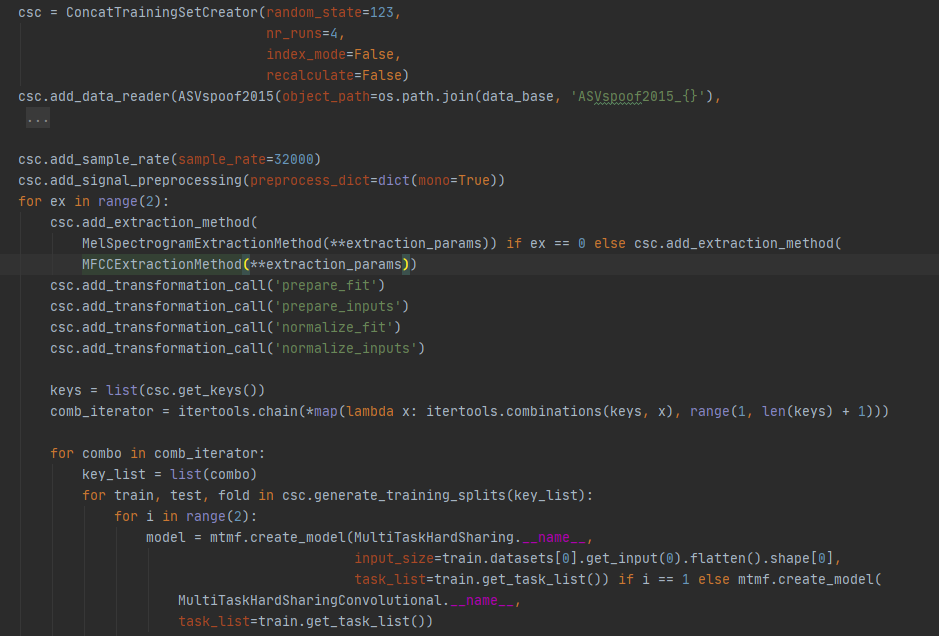
\includegraphics[width=\linewidth]{screenshot005}
	\caption{Data Loading in the variation experiments}
	\label{fig:screenshot005}
\end{figure}

% TODO: Expand on which datasets and what tasks
In total 7 datasets were used in creating this set-up, with 8 tasks. The dataset linked to two tasks is the same used earlier for \citep{georgiev2017low}. The tasks contain both multi-class and multi-label tasks. Each combination is tested for 2 extraction methods and 2 models. For each run, the feature matrices should be framed in the same size, based on the average feature matrix size and the data normalized. As can be seen in table \ref{table:LOC}, this is the first time the required Training LOC makes a significant jump in the Training stage, simply due to the fact that it varies models. The models are loaded for the first time through the MultiTaskModel factory which mainly functions as a way to concentrate static and dynamic model parameters for creation and isn't absolutely necessary. Otherwise, the training is performed using the same three lines as before: model creation, results creation and training loop instantiation. The Data Loading stage also takes a jump, but is in no way related to the high and diverse amount of datasets, simply the variation of elements in the pipeline. There are  operations performed in the pipeline: resampling, conversion to mono, calculating and framing the feature matrices, normalizing the data. The Data loading code can be found in figure \ref{fig:screenshot005}, which makes it apparent that the extra lines outside the transformation calls are simply due to iterating over the required variations. The actual amount of LOC relating to direct data loading operations is 8.\\

This example makes it clear that all the work concerning datasets comes beforehand in the Data Reading stage, with little extra effort on the developer's side, while the combinatorial aspects are handled by the framework in the background. Nothing has to be explicitly reloaded or recalculated, as seen when adding the ExtractionMethod, by the developer as variations will be handled by the framework and necessary data recalculated when required. The framework thus reduces research variations to singular line changes.\\

To build on the last point of reducing work for research variations, especially in future work, it should be noted that given that the previous implementations would have been made as was the case in this scenario, only two extra datasets were added: FSD Kaggle 2018 TODO: REFERENCE and the Speech Commands dataset TODO: Reference. Given that, the Data Reading would be reduced to 8 + 83 LOC in this implementation. DataReader objects are merely paths for extracting the data, while the specifics of how can be given later. Vanilla implementations would either require large code changes if e.g. other extraction methods or signal preprocessing functions were required or have to take these in account beforehand and likely end up with similar structures. \\


\begin{figure}
	\centering
	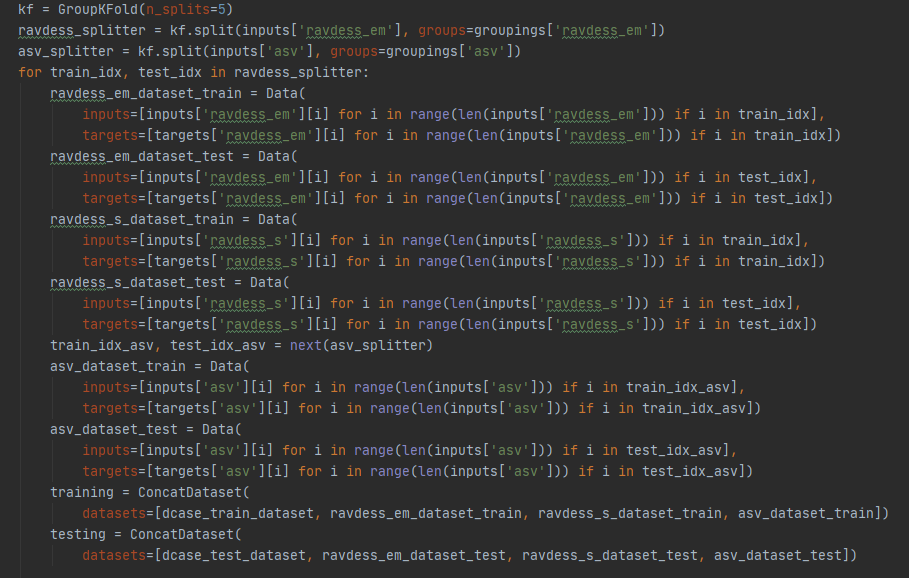
\includegraphics[width=\linewidth]{screenshot002}
	\caption{Train and Test set creation without framework for the \cite{georgiev2017low} implementation}
	\label{fig:screenshot002}
\end{figure}

\begin{figure}
	\centering
	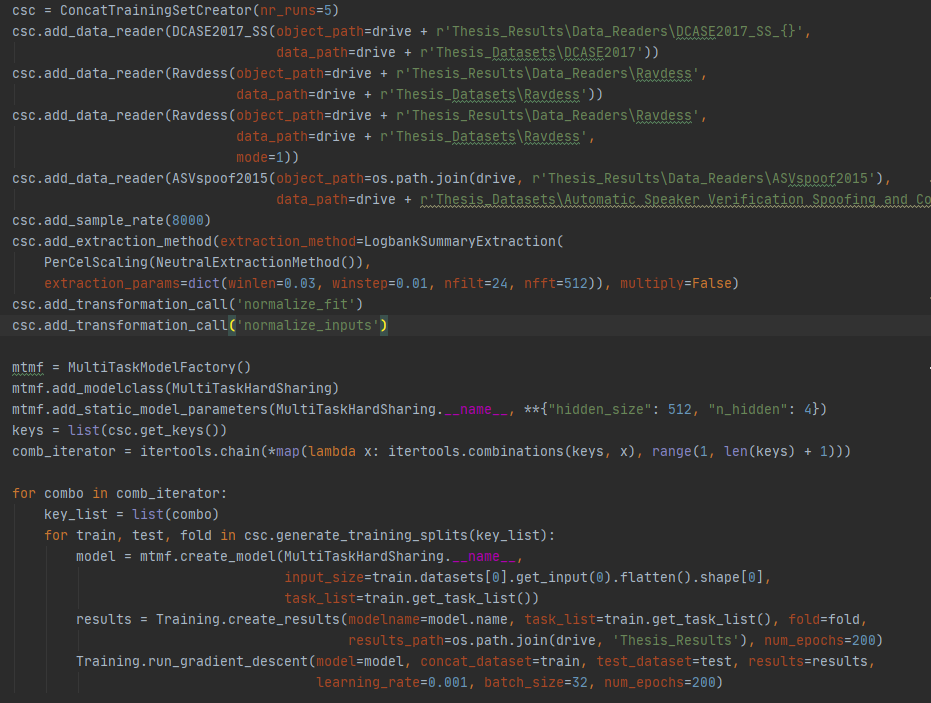
\includegraphics[width=\linewidth]{screenshot003}
	\caption{Complete implementation of \cite{georgiev2017low} with the framework}
	\label{fig:screenshot003}
\end{figure}

What these efforts demonstrate is that the LOC only directly scale with added required operations and do not spill over in other stages. To clarify the last part, figures \ref{fig:screenshot002} illustrate how without the framework, train and test set generation - which falls under the data loading stage - scales directly depending on the amount of datasets used. Compare that to figure \ref{fig:screenshot003}, where it can be seen that train and test generation is actually reduced to one simple line before the three Training stage lines in the end. This also demonstrates how the framework grants flexibility in which datasets to actually load and split with the key\_list input, which grants further work reduction as in practice it is possible that not all datasets are required which were planned beforehand. In the first case, that would imply multiple lines of code change, while in the second, simply one line for the key list. \\

What should again be noted, is that the implementations without the framework did not include a lot of the extra features that are performed automatically, the main one being quick reading and writing of the data. To reiterate, this means that when the Data Reading stage is done, it is written to files on the disk, so that future runs would not unnecessarily have to reextract feature matrices. Including these would raise the LOC required for the vanilla implementations a lot and would either have specific implementations per dataset or end up constructing similar functions to the framework. These LOC comparisons are for the bare required necessities only.\\



%\begin{table}[ht]
%	\caption{Reported metric comparisons} % title of Table
%	\centering % used for centering table
%	\begin{tabular}{p{0.25\textwidth}p{0.25\textwidth}p{0.25\textwidth}p{0.25\textwidth}} % centered columns (4 columns)
%		\hline\hline %inserts double horizontal lines
%		Title & Metric & Reported & Implementation  \\ [0.5ex] % inserts table
%		%heading
%		\hline % inserts single horizontal line
%		\citet{park2020augmenting} & Precision & 0.796 & 0.7741 \\ \hline
%		\citet{park2020augmenting} & Recall & 0.804 & 0.763  \\ \hline
%		\citet{park2020augmenting} & F1 Score & 0.8 & 0.7685 \\ \hline
%		\citet{xu2019multi} & Unweighted Average Recall & 0.662 & 0.6716 \\ \hline
%	\end{tabular}
%	\label{table:metric} % is used to refer this table in the text
%\end{table}
%
%Following the example from other deep learning frameworks like \cite{colacco2020drecpy} it is important that the framework demonstrates to be consistent with published results. In table \ref{table:metric} the comparative results can be found with the original publications. The decision was made to focus on the best reported performance of the multi-task setting, in order to limit the amount of work time to reproduce some of the results. Papers are often incomplete when it comes to specifics required to reproduce the same elements which can impact the results considerably, which requires careful variation and evaluation of the parameters.\\
%
%Starting from the top, the results from the classifier built in \cite{park2020augmenting} come close but slightly below the reports. Multiple node amounts in the DNN were tried, as the original paper lacked to include the exact after the initial layer, yet implying the amount lessen through the figure included. Furthermore, the exact included instances are not the same. The work mentions some cleaning of the dataset was performed, but neglect to mention the specifics. The result is the best performing variation. The amount of nodes was halved in the final two layers and minimal logical clean up was performed (e.g. an audio fragment can not have both silence and another label at the same time). Still, the eventual results end up relatively close to the report.\\
%
%???????????????????????

%Toon in use case met experiment hoe ge een variatie kunt maken aan 1 element in de pijplijn, terwijl de rest intact blijft
\section{Experiment use case}

%- Describe the goal of making a huge functioning multi-task network
% Describe the steps of iterative design, demonstrating how single line changes can be made while keeping the rest of the pipeline intact
% Demonstrate the comparative capabilities in tensorboard
% Analysis: implementing baseline 
% iterative design of classifier
% variation of meta parameters
% 
% architecture
% design
% construction
% testing
% deployment
% maintenance
%- Testing different variations
%- finding the meta parameters
% comparing to baseline

%THings that it demonstrates
% How elements can be added and changed at will at any point
% - Meta parameter search
% - Architecture evaluation
% - Expanding the dataset
% How testing can be done
% - How baseline tests can be performed by bringing in previous models 
% - How comparative visualizations can be made and accessed

% Add datasets
% simple model structure
% build pipeline
% create validation set
% test architecture and 
% evaluate
% loop to test meta parameters
% Evaluate
% Run eventual test and training


Additional to the paper implementations, is an example case study which has been referred to multiple times in this work. The goal is to present how the framework aids the development of multi-task systems by conducting a development process. As stated in \cite{brown1996framework}, this form of evalution is "intended to reveal the broader charactersistics of a technology when it is applied to a representative “complete” problem in an application domain". This case study involves developing a multi-task, multi-dataset neural network  \\



\section{Literature Evaluation}

%TODO: Dive in the literature and describe its implementation on the software, which components can be adjusted or nah

In line with the goal to provide a tool that can spur development of multi-task research, this section will examine the papers identified in tables \ref{table:combinations}, \ref{table:combinations2}, \ref{table:combinations3} in order to evaluate the expressiveness of the framework as well as its limitations. Specifically, the examination will be made in terms of changes that are required to achieve some of the necessary features. \\

% Make table with things that require big changes (i.e. the core)
% Make a table with things that require extensions
% Make a table that overviews the possible/not possible





\section{Fulfilment of the Requirements}

\subsection{Non-functional Requirements}
\begin{itemize}
	\item \textbf{Modular:} 
	%	Demonstrate the replaceability in the code
	\item \textbf{Extendible:} 
	%	Extensibility is discussed in design section
	\item \textbf{Fast prototyping:} 
	% Demonstration implementations, comparison with implementation without
	\item \textbf{Cutting Double Work:} 
	% Demonstration of the research set-up
%	\item \textbf{Developmental Side-rails:}
%	%  
	\item \textbf{Flexible:} 
%	Demonstration + Dive in the literature

\end{itemize}

\subsection{Funtional Requirements}
\subsubsection{Data Reading}
\begin{itemize}
	\item Standardizing Input - The TaskDataset object is developed for assuring that the data is valid throughout the rest of the process. Its extension of PyTorch's Dataset class ensures that it can be utilised by the PyTorch framework. The builder pattern allows the TaskDataset to be built incrementally and valid along the way, with each step including various validity checks.
	The exception where the TaskDataset can't check for validity is in terms of the input feature matrix size. The matrix sizes might not be compatible with the developed PyTorch Model. The responsibility for this is up to the developer.
	% How do we know this works?
	% What validity checks?
	\item Handling dataset differences - The DataReader class is an abstract class that the developer must extend to deal with the peculiarities of navigating each dataset structure to extract the correct information. This corresponds to it being a white box hot-spot. Predefined train/test splits can be stored through the HoldTaskDataset structure and pre-split audio segments can be kept together by defining the grouping. 
	% Refer to the implementations for differences
	\item Scalable preprocessing - Preprocessing audio signals and preprocessing feature matrices happen in different places, as TaskDatasets should only contain valid input instances at any point. Preprocessing signals can utilise an (optional) function from the DataReader class with parameters that are received when the TaskDataset is extracted. Reusing the method can thus hand developers easy replicability of the signal preprocessing. These can be further scaled by using the TrainingSetCreator. In this class, any preprocessing or transformation can be added 'on the fly'. This means that if a functionality (e.g. resampling) is added, any previous 
	% What preprocessing do we have for both signals and feature matrices
	\item File storage abstraction: There are handles on the TaskDataset which can be called to store, load or check the TaskDataset to or from files, which are specific for the currently used extraction method and task.
	\item Quick Reading: The DataReader automatically checks if there is a stored TaskDataset available for the given extraction\_method and task and loads it if so.
	\item Create multiple input objects from the same dataset: (DEMONSTRATE) The framework is open ended in how the TaskDataset object is extracted from the data and allows extra parameters for the DataReader to be given at initialization. TaskDatasets are stored using the ExtractionMethod object's name and the (main) Task's name, so for every new variation of these will be automatically linked to different files.
	\item Tasks and datasets are a many to many relationship: Tasks can be present in multiple datasets. The tasks need to have the same name, output labels and classification type in order to be seen as the same. When combined in the ConcatTaskDataset, the target vectors will automatically be placed in the same positions, which will make them be seen as the same task in the training function. Datasets can have multiple tasks to an unlimited degree in its list of extra tasks, which always combines them with a list of targets of the same amount of input instances. 
\end{itemize}
\subsubsection{Data Loading}
\begin{itemize}
	\item Combining datasets: Extended the ConcatTaskDataset, extra functions for the batching
	\item Not requiring the combined datasets in memory:  Index mode implemented which forms a streaming context for the data to be stored and read from disk.
	\item Train and test set generation: They implemented through the HoldTaskDataset
	\item Transforming data: They implemented through handles on the TaskDataset which call upon the ExtractionMethod
	\item Filtering data: Handle on the TaskDataset
	\item Reusing data: It implemented, reusability is possible without reloading to different degrees
	\item Batching multiple tasks: It implemented lol
	\item Replicability: It implemented through storing the different checkpoints (which can be recreated by reloading the Results object), the calculation data in extractionmethods and 
	\item Scalable Manipulation: In the TrainingSetCreator, manipulations can be added for one specified dataset or all at once.
\end{itemize}
\subsubsection{Training}
\begin{itemize}
	\item Predicting multiple tasks: Each dataset can have multiple tasks linked to their targets. There are automatic filters for the output to isolate the task specific predictions. 
	\item Task specific output handling: Handling of the task functions, like loss calculation and decision making of the eventual classes from the probabilities are stored in the Task objects 
	\item Loss calculation specifiable: The calculation of the Loss of each task is definable in the Task object. However, currently, losses are always tied to tasks, which have target labels. This is not always the case, as in the research \citep{tagliasacchi2020multi} \citep{wu2020domain}, losses have also been calculated based on cost functions from internal model parameters. Since these loss functions are not linked to datasets, but to the models themselves, for which the framework does not offer modules which can be used in the training function for specific handling, it is up to the developer to implement these in the Training\_Utils object.
	\item Loss combination specifiable: Implemented in the Training\_Utils object
	\item Metric calculation, storage and visualization: Gives predictions, true labels and losses to the Results object which calculates the metrics, stores them and writes them to tensorboard where they can easily be compared to other results
	\item Interrupted Learning: (DEMONSTRATE) Implemented by recreating the Results object and starting the training loop from the given epoch.
	\item Separate evaluation: (DEMONSTRATE) The evaluation function is separate from the training loop. Training parameters for transformations and such can be reloaded from the stored extraction\_method object as well as the model parameters at every epoch in the training function. 
	\item Direct comparison of different runs: Every run has a unique name and TensorBoard has the ability to place the results from different files side-by-side
	\item Variable training paradigms: In this state, the only training paradigm available is Gradient Descent. Implementing a different paradigm requires foregoing the current training loop implementation.
\end{itemize}
	\chapter{Conclusion}

\section{Future Work} %3 pages

	
	
\bibliographystyle{plainnat} 
%\bibliographystyle{plain} 
%\bibliographystyle{IEEEtranN} 
\bibliography{references}
	
\end{document}         